\documentclass{article}
\usepackage{amsfonts, amsmath, amssymb, amsthm, dsfont} % Math notations imported
\usepackage{enumitem}
\usepackage{graphicx}
\usepackage{setspace}
\usepackage{indentfirst}
\usepackage[margin=1in]{geometry}
\graphicspath{{./images/}} % Path to images

% \begin{figure}[htb!]
%      \centering
%      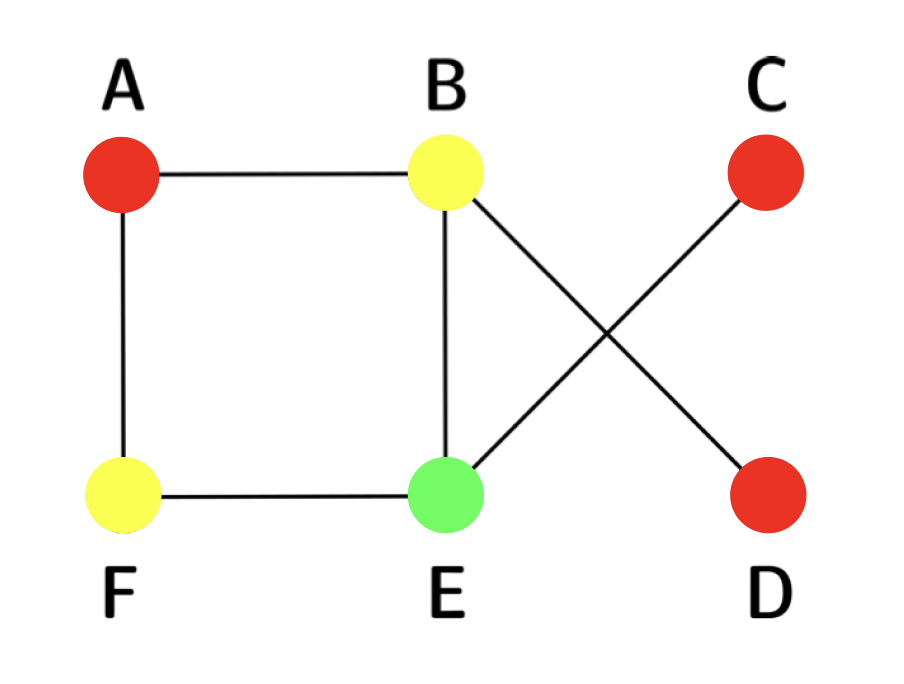
\includegraphics[scale=0.5]{coloring.png}
%      \caption{Coloring of the graph.}
% \end{figure}

% \begin{figure}[htb]
%     \qquad
%     \begin{minipage}{.4\textwidth}
%         \centering
%         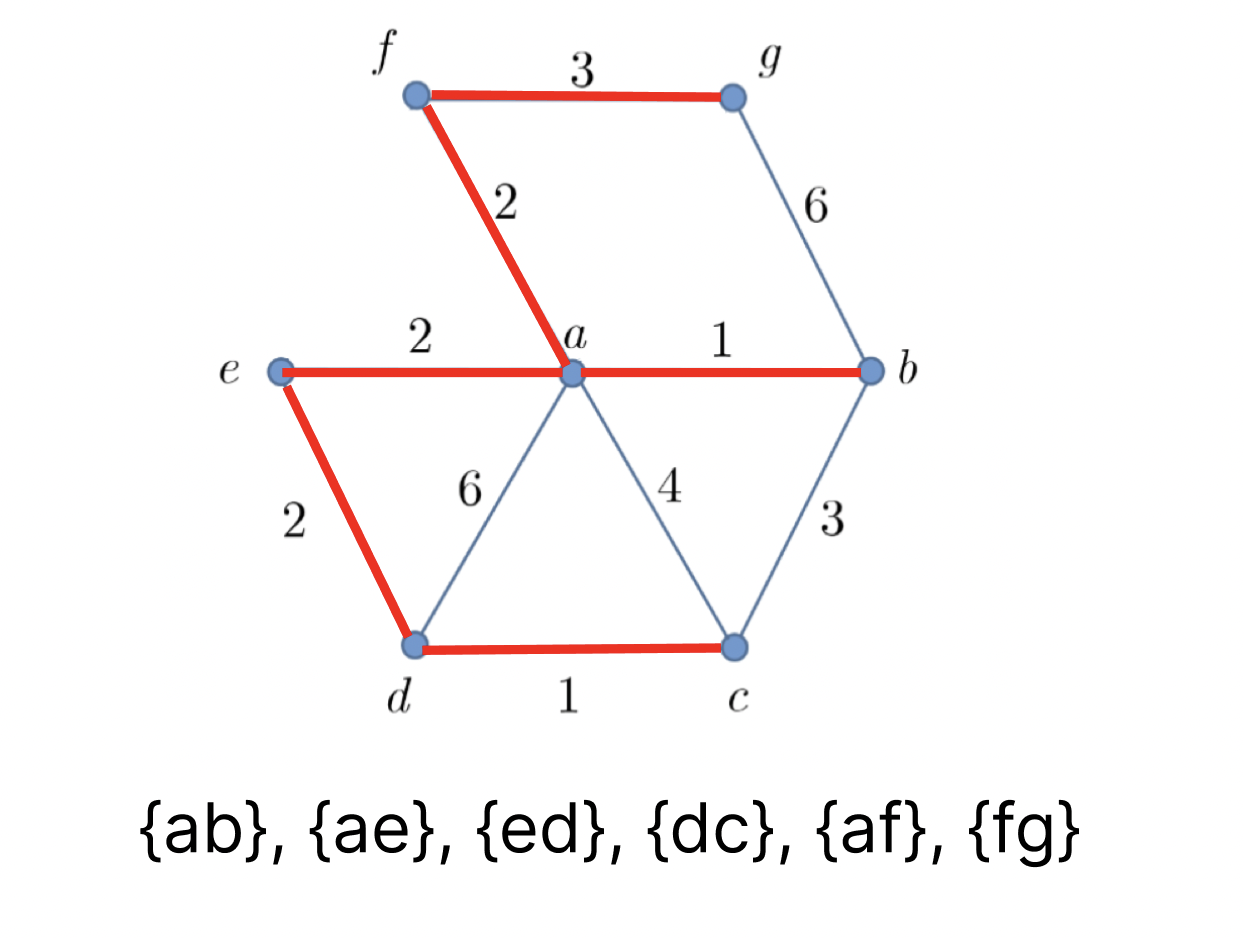
\includegraphics[scale=0.35]{prims.png}
%         \caption{}
%     \end{minipage}    
%     \qquad
%     \begin{minipage}{.4\textwidth}
%         \centering
%         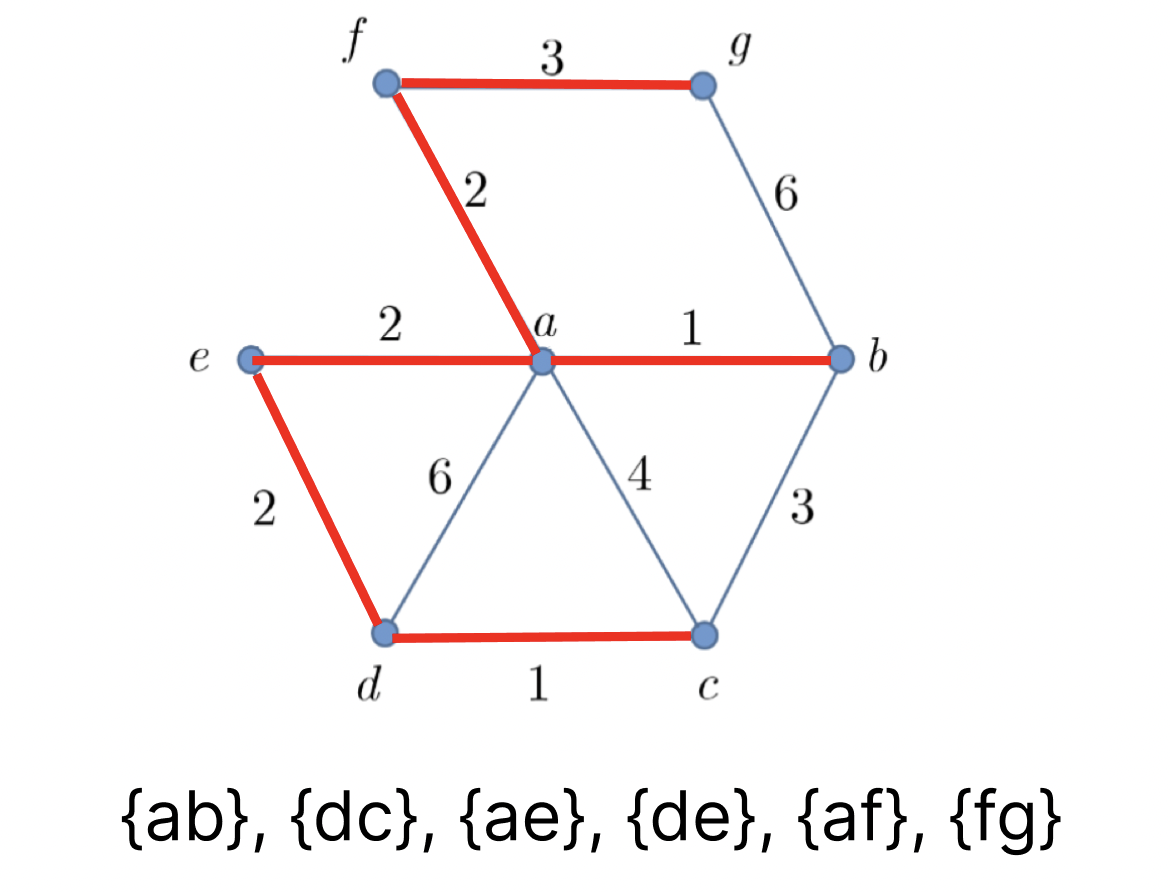
\includegraphics[scale=0.35]{kruskal.png}
%         \caption{}
%     \end{minipage}        
% \end{figure} 

\newtheorem{thm}{Theorem}
\newtheorem{proposition}[thm]{Proposition}
\newtheorem{corollary}[thm]{Corollary}
\newtheorem{lemma}[thm]{Lemma}

\newcommand*{\Var}{\ensuremath{\mathrm{Var}}}
\newcommand*{\Cov}{\ensuremath{\mathrm{Cov}}}
\newcommand*{\Corr}{\ensuremath{\mathrm{Corr}}}
\newcommand*{\Bias}{\ensuremath{\mathrm{Bias}}}
\newcommand*{\MSE}{\ensuremath{\mathrm{MSE}}}
\newcommand*{\range}{\ensuremath{\mathrm{range}}\,}
\newcommand*{\spann}{\ensuremath{\mathrm{span}}\,}
\newcommand*{\nul}{\ensuremath{\mathrm{null}}\,}
\newcommand*{\dom}{\ensuremath{\mathrm{dom}}\,}
\renewcommand*{\implies}{\ensuremath{\Longrightarrow}}
\renewcommand*{\impliedby}{\ensuremath{\Longleftarrow}}
\newcommand*{\Z}{\ensuremath{\mathbb{Z}}}
\newcommand*{\Q}{\ensuremath{\mathbb{Q}}}
\newcommand*{\R}{\ensuremath{\mathbb{R}}}
\newcommand*{\F}{\ensuremath{\mathbb{F}}}
\newcommand*{\C}{\ensuremath{\mathbb{C}}}
\newcommand*{\N}{\ensuremath{\mathbb{N}}}
\newcommand*{\E}{\ensuremath{\mathds{E}}}
\renewcommand*{\P}{\ensuremath{\mathds{P}}}
\newcommand*{\p}{\ensuremath{\mathcal{P}}}

% title information
\title{Math 110 HW10}
\author{Neo Lee}
\date{11/11/2023}

\setstretch{1.15}
% main content
\begin{document} 

% placing title information; comment out if using fancyhdr
\maketitle 

\subsection*{Problem 1.}
Determine whether or not the function taking the pair $((x_1,x_2,x_3),(y_1,y_2,y_3)) \in \R^3 
\times \R^3$ to $x_1y_1+x_2y_2-3x_2y_3+3x_3y_2+x_3y_3$ is an inner product. 
\begin{proof}
    \textbf{Conjugate symmetry:} Let $u=(1,2,3), v=(4,5,6)$,
    \begin{align*}
        \langle u,v\rangle & = 1\times 4 + 2\times 5 + 3\times 6 - 3\times 2\times 6 + 3\times 3\times 5 \\
        & \neq 1\times 4 + 2\times 5 + 3\times 6 - 3\times 3\times 5 + 3\times 2\times 6 = \langle v, u\rangle.
    \end{align*}

    Hence, the function is not an inner product.
\end{proof}

\newpage
\subsection*{Problem 2.}
Consider a complex vector space $V={\rm span}\, (1, \cos x, \sin x, \cos 2x, \sin 2x)$ with 
an inner product $$\langle f,g\rangle := \int_{-\pi}^{\pi} f(t)\overline{g(t)} dt.$$  
Let $U$ be the subspace of odd functions in $V$. What is $U^\perp$? Find an orthonormal 
basis for both $U$ and $U^\perp$. 
\begin{proof}
    We have proved previously in the midterm exam that $$U = \spann\{\sin x, \sin 2x\}.$$ Then, notice 
    the set $\{1, \cos x, \cos 2x\}\perp U$ because let $f(t)\in U$ and $g(t)\in
    \{1, \cos x, \cos 2x\}$, then $f(t)\overline{g(t)}$ is an odd function because $f(t)$ is odd while 
    $\overline{g(t)}=g(t)$ is even, hence $\int_{-\pi}^{\pi}f(t)\overline{g(t)}dt = 0$.

    Notice $\spann\{1,\cos x, \cos 2x\} \subseteq U^\perp$ because any $w\in U^\perp$ can be written as a 
    linear combination of $\{1,\cos x, \cos 2x\}$, and by linearity of integration, the inner product with any 
    $u\in U$ is 0.

    In fact, $\spann\{1,\cos x, \cos 2x\} = U^\perp$ because $$\dim U^\perp = \dim V - \dim U = 5-2=3$$
    and $\dim\spann\{1,\cos x, \cos 2x\}=3$.
\end{proof}

\newpage
\subsection*{Problem 3.}
Consider the space ${\cal P}_3(\R)$ with the inner product
$$ \langle f, g \rangle = \int_{-1}^1   f(x) g(x) dx. $$
Use the Gram-Schmidt algorithm to orthonormalize the basis $1,x,x^2,x^3$.
\begin{proof}[Solution]
    \begin{align*}
        e_1 & = \frac{1}{\sqrt{\langle1,1\rangle}} = \frac{1}{\sqrt{2}} \\
        e_2 & = \frac{x-\langle x,e_1\rangle e_1}{\|x-\langle x,e_1\rangle e_1\|} \\
        & = \frac{x-\frac{1}{\sqrt{2}}\int_{-1}^{1}\frac{x}{\sqrt{2}}dx}
        {\|x-\frac{1}{\sqrt{2}}\int_{-1}^{1}\frac{x}{\sqrt{2}}dx\|} \\
        & = \frac{x-0}{\|x-0\|} \\
        & = \frac{x}{\sqrt{\int_{-1}^{1}x^2dx}} \\
        & = \frac{x}{\sqrt{2/3}} = \sqrt{\frac{3}{2}}x \\
        e_3 & = \frac{x^2-\langle x^2,e_1\rangle e_1-\langle x^2,e_2\rangle e_2}
        {\|x^2-\langle x^2,e_1\rangle e_1-\langle x^2,e_2\rangle e_2\|} \\
        & = \frac{x^2-\frac{1}{\sqrt{2}}\int_{-1}^{1}\frac{x^2}{\sqrt{2}}dx
        -\frac{3}{2}x\int_{-1}^{1}x^3dx}
        {\|x^2-\frac{1}{\sqrt{2}}\int_{-1}^{1}\frac{x^2}{\sqrt{2}}dx
        -\frac{3}{2}x\int_{-1}^{1}x^3dx\|} \\
        & = \frac{x^2-1/3}{\|x^2-1/3\|} \\
        & = \frac{x^2-1/3}{\sqrt{8/45}} \\
        e_4 & = \frac{x^3-\langle x^3,e_1\rangle e_1-\langle x^3,e_2\rangle e_2
        -\langle x^3,e_3\rangle e_3}
        {\|x^3-\langle x^3,e_1\rangle e_1-\langle x^3,e_2\rangle e_2
        -\langle x^3,e_3\rangle e_3\|} \\
        & = \frac{x^3-\frac{1}{\sqrt{2}}\int_{-1}^{1}\frac{x^3}{\sqrt{2}}dx
        -\frac{3}{2}x\int_{-1}^{1}x^4dx-\frac{x^2-1/3}{\sqrt{8/45}}\int_{-1}^{1}x^3\left(\frac{x^2-1/3}{\sqrt{8/45}}\right)dx}
        {\|x^3-\frac{1}{\sqrt{2}}\int_{-1}^{1}\frac{x^3}{\sqrt{2}}dx
        -\frac{3}{2}x\int_{-1}^{1}x^4dx-\frac{x^2-1/3}{\sqrt{8/45}}\int_{-1}^{1}x^3\left(\frac{x^2-1/3}{\sqrt{8/45}}\right)dx\|} \\
        & = \frac{x^3-\frac{3}{2}x\cdot\frac{2}{5}}{\|x^3-\frac{3}{2}x\cdot\frac{2}{5}\|} \\
        & = \frac{x^3-\frac{3}{5}x}{\sqrt{\int_{-1}^{1}(x^3-\frac{3}{5}x)^2dx}} \\
        & = \frac{x^3-\frac{3}{5}x}{\sqrt{8/175}}.
    \end{align*}
\end{proof}

\newpage
\subsection*{Problem 4.}
Let $e_1$, $\ldots$, $e_m$ be an orthonormal list of vectors. Prove that
$v\in \spann (e_1,\ldots, e_m)$ if and only if
$$ \| v\|^2 = \sum_{j=1}^m |\langle v, e_j\rangle |^2.$$
\begin{proof}
    The forward direction falls directly from \emph{Theorem 6.30 (b)} where
    $V=\spann\{e_1,\dots, e_m\}$. 
    
    For backward direction, assume 
    $\| v\|^2 = \sum_{j=1}^m |\langle v, e_j\rangle |^2$ but $v\not\in\spann(e_1,\dots,e_m)$. Now, we 
    take the smallest vector space containing $v$ and write out its basis as $(v_1, \dots, v_n)$, where
    there are some $v_j\not\in(e_1,\dots, e_m)$. We take those basis and append to 
    $(e_1,\dots, e_m)$ to get $(e_1,\dots, e_m, v_j,\dots)$.
    Then we apply Gram-Schmidt algorithm to $(e_1,\dots, e_m, v_j,\dots)$ to get a new orthonormal 
    basis $(e_1,\dots, e_m, w_j,\dots)$, which has the same span as $(e_1,\dots, e_m, v_j,\dots)$. 
    Therefore, $v$ can be written as a linear combination of this new basis, i.e.
    $$v = \underbrace{a_1e_1 + \cdots + a_m e_m}_u + \underbrace{b_jw_j,\dots}_w,$$
    where $w$ is orthogonal to $u$ and is non-zero. Then by the \emph{Pythagorean Theorem}, we have
    $$\|v\|^2 = \|u\|^2 + \|w\|^2 > \|u\|^2 = \sum_{j=1}^m |\langle v, e_j\rangle |^2,$$
    which is a contradiction. Hence, $v\in\spann(e_1,\dots, e_m)$.
\end{proof}

\newpage
\subsection*{Problem 5.}
Suppose that $e_1$, $\ldots$, $e_n$ is a list of vectors in $V$ of length $1$ (i.e., $\|e_k\|=1$
for all $k=1,\ldots, n$) such that
$$\|v\|^2=|\langle v,e_1\rangle |^2+\cdots + |\langle v, e_n  \rangle|^2 \quad  {\rm for \; all} \;\; v\in V.$$
Prove that $e_1$, \ldots, $e_n$ is an orthonormal basis of $V$.
\begin{proof}
    First, we show that $(e_1,\dots, e_n)$ is orthogonal. Take $v=e_j$ for some $j\in\{1,\dots, n\}$, 
    then put in the equation, we see that
    \begin{align*}
        \|e_j\|^2 & = |\langle e_j, e_1\rangle|^2 + \cdots + |\langle e_j, e_j\rangle|^2
        +\cdots + |\langle e_j, e_n\rangle|^2 \\
        1 & = |\langle e_j, e_1\rangle|^2 + \cdots + 1
        +\cdots + |\langle e_j, e_n\rangle|^2,
    \end{align*} which means $|\langle e_j, e_i\rangle|^2 = 0 \implies \langle e_j, e_i\rangle=0$ for $i\neq j$.
    Since $e_i$ all have unit length, they are orthonormal. Then from \emph{Problem 4}, we know that
    $v\in\spann(e_1,\dots,v_n)$ for all $v\in V$. In other words, $(e_1,\dots, e_n)$ span the entire 
    vector space $V$. At the same time, they are orthogonal hence linearly independent. Therefore,
    $(e_1,\dots, e_n)$ is a basis, in particular orthonormal basis, of $V$.
\end{proof}

\end{document}
